\section{Microservices and availability}

Consider the microservice-based architecture shown in the figure below. 
The architecture is organized in eight stateless microservices that collaborate to fulfill requests R1 and R2. 
S1 is the front-end service that receives both requests. 
The fulfillment of request R1 requires the interaction with services S2 and S3 (through sub-requests R1.1 and R1.2, respectively), which, in turn, need to interact with other services. 
In particular, S2 interacts with S4 and S5 and S3 with S5 and S6.
The fulfillment of R2 requires that S1 interacts with S8 which, in turn, interacts with S6 and S7.
\begin{figure}[H]
    \centering
    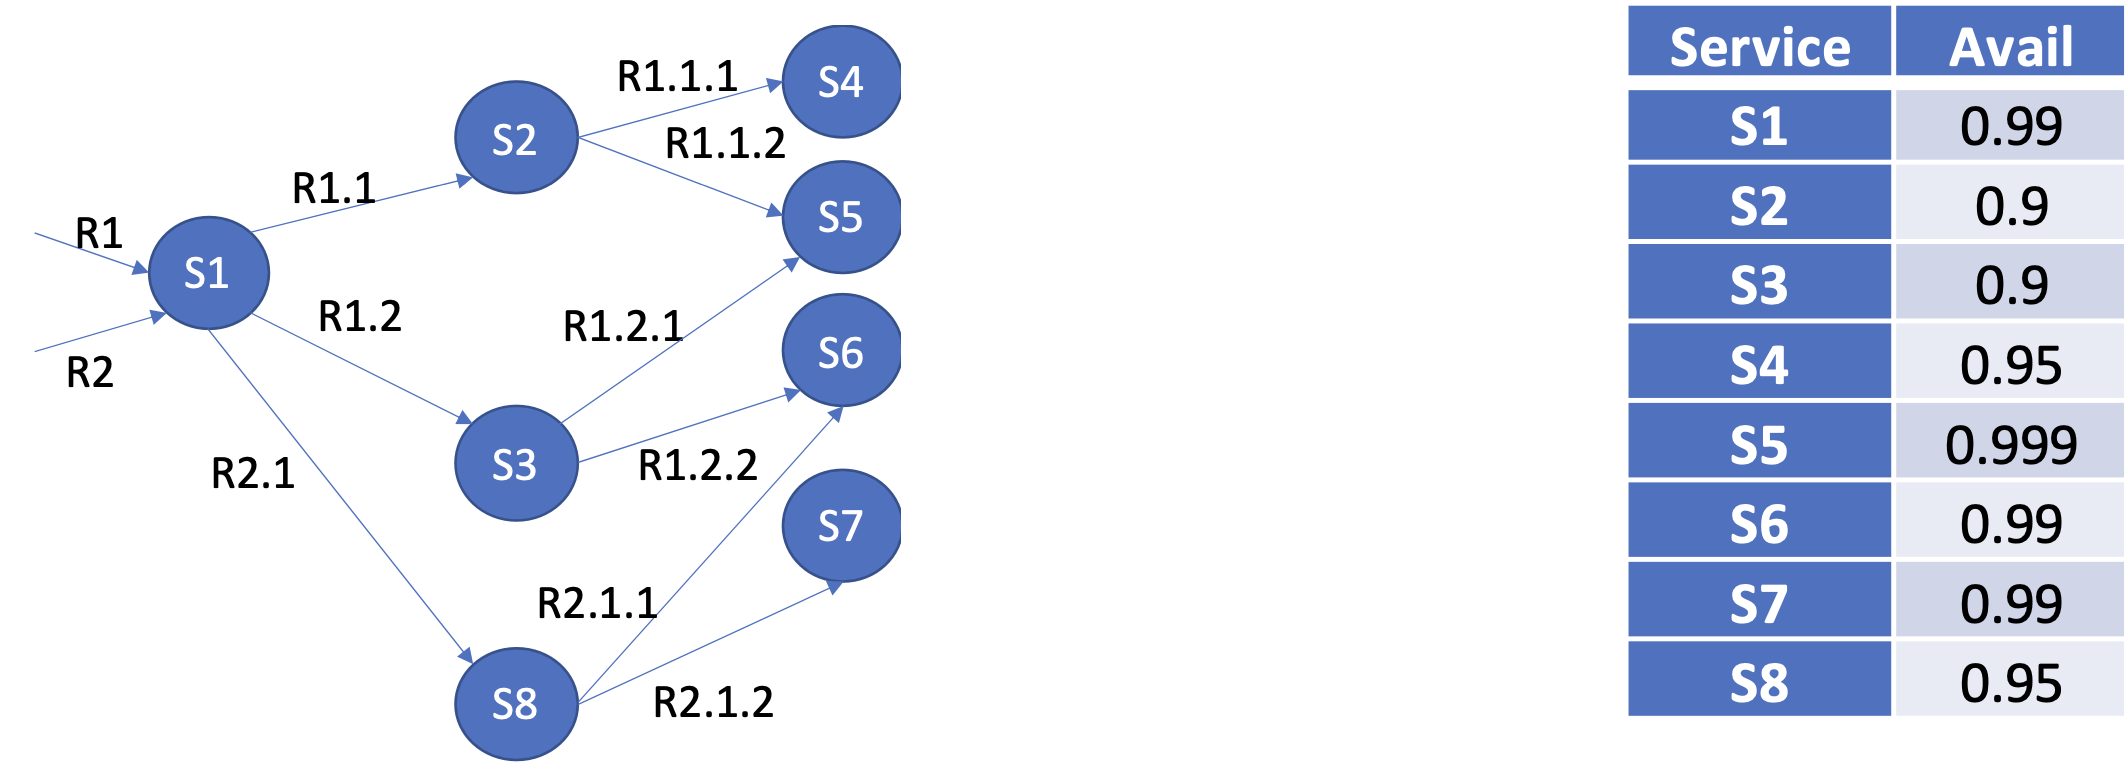
\includegraphics[width=0.9\linewidth]{images/micro.png}
\end{figure}
\begin{enumerate}
    \item Assuming that the availability of services S1-S8 is the one reported in the table above, what is the availability of the system when answering to request R1?
    \item If each of the services S1-S8 is duplicated, what is the new value of the availability computed at point 1?
\end{enumerate}

\paragraph*{Solution}
\begin{enumerate}
    \item Note that, regardless of the way the interaction between the \texttt{MessageQueue} and the DataAnalyzer works, data have to flow through the whole chain of components to be processed. 
        This implies that we can model the system as a series of component.
        The total availability of the system is determined by the weakest element, that is, the \texttt{DataCollector}.
        \[A_{\text{Total}} = 0.99 \cdot 0.9999 \cdot 0.995 = 0.985\]
        If we parallelize the data collector adding a new replica, we can achieve the following availability:
        \[(1-(1-0.99)2) \cdot 0.9999 \cdot 0.995 = 0.995\]
        At this point, even if we increase the number of \texttt{DataCollector} replica, we do not achieve an improvement as the weakest component becomes the DataAnalyzer.
        We can parallelize this component as well to further improve the availability of our system.
    \item Let's consider the impact of the \texttt{DataCollector} parallelization on the rest of the system.
        If both replicas acquire information from the same sources in order to guarantee that all data are offered to the rest of the system, then the other components will see all data duplicated and will have to be developed considering this situation. 
        For instance, the \texttt{MessageQueue} could discard all duplicates. 
        Another aspect to be considered is that both \texttt{DataSources} and \texttt{MessageQueue} have to implement mutual exclusion mechanisms that ensure the communication between them and the two \texttt{DataCollector} replicas does not raise concurrency issues. 
        Another option could be that only one \texttt{DataCollector} replica at a time is available, and the other is activated only when needed (for instance, if the first one does not send feedback within a certain timeout).
\end{enumerate}

